% 原书印刷177--183页，PDF物理201--207页，止于5.2标题之前.
本章将利用两个概率测度之间运输问题的最小值，在概率测度空间上定义距离. 主要考虑$\Omega\subset\mathbb R^d$中形如$c(x,y)=|x-y|^p$的成本，但分析也可调整到更一般度量空间$X$中距离的幂. 为利用$L^p$范数的性质，始终取指数$p\in[1,+\infty[$（将在讨论部分\autoref{sec:5.5.1}简要介绍$p=+\infty$）. 当$\Omega$无界时，需要将分析限制于以下概率测度集合：
\[
\mathscr P_p(\Omega):=\left\{\mu\in\mathscr P(\Omega):\int_\Omega|x|^p\,d\mu<+\infty\right\}.
\]
在度量空间中，固定任意一点$x_0\in X$，令$\mathscr P_p(X):=\{\mu\in\mathscr P(X):\int d(x,x_0)^p\,d\mu(x)<+\infty\}$（该积分是否有限与$x_0$的选择无关）.

暂不深入细节，只说明所用距离如下定义：对$\mu,\nu\in\mathscr P_p(X)$，令$W_p(\mu,\nu):=\mathscr T_c(\mu,\nu)^{1/p}$，其中$\mathscr T_c$是成本$c(x,y)=d(x,y)^p$的最小运输成本，$d$为$X$上的距离.

这样得到的距离称为\emph{Wasserstein距离}（Wasserstein distance）.\footnote{这一名称很有争议，尤其在俄罗斯，因为在美国工作的俄罗斯学者L.~Vaserstein（其名字有时拼作Wasserstein），实际上并没有在引入这些距离时发挥人们可能想象的关键作用. 然而，如今这是西方国家的标准名称，很可能源于\cite{b198,b246}中采用的术语；即使经常有人建议使用Monge--Kantorovich距离等其他名称，这一惯例似乎也已无法改变. \phantomsection\label{idx:root5-p177-emd}\index{E048@推土机距离（Earth Mover Distance）|hyperpage}另请注意，在偏应用的群体中，这一距离也常称为Earth Mover Distance（EMD，推土机距离）.}它们在许多应用领域十分重要，似乎是描述同一空间上等量质量分布之间距离的一种自然方式. 用对应用更有意义的语言来讲，\footnote{特别是在图像处理中. 感谢G.~Peyré指出这一解释.}可以说，Wasserstein距离从物体（颜色、词语、点等）的集合$X$上的一个距离出发，在$X$上所有可能的直方图的集合上产生一个距离（另见\autoref{sec:2.5.1}）.

将这些距离与密度之间的$L^p$距离比较很有意思（例如，对$\mathbb R^d$上的绝对连续测度，这种比较有意义）. 首先可观察到，这两类距离的行为非常不同. 可以说，若$L^p$距离是“竖直的”，Wasserstein距离就是“水平的”. 这种说法很不正式，但若将每个绝对连续测度与其密度的图像相联系，就十分自然. 为计算$\|f-g\|_{L^p}$，需对每一点$x$考察$f(x)$与$g(x)$的距离，对应于两个图像之间的竖直位移，再对该量积分. 相反，为计算$W_p(f,g)$，需要考虑点$x$与点$T(x)$之间的距离（即图像上的水平位移），再对它积分；这里$x$与$T(x)$按某种特定方式配对，从而构成$f$与$g$之间的一个耦合.

以下第一个例子说明两种距离计算方式的行为差异很大：取支撑于$[0,1]$的两个密度$f$与$g$，定义$g_h(x)=g(x-h)$. 只要$|h|>1$，$f$与$g_h$之间的$L^p$距离就等于$(\|f\|_{L^p}^p+\|g\|_{L^p}^p)^{1/p}$，与$|h|$这一“空间”信息无关. 相反，$f$与$g_h$之间的$W_p$距离具有$|h|$的量级（当$h\to\infty$时），与$f$、$g$的形状相比，它对位移的依赖强得多. 再考虑密度$g$与其平移$g_h$之间的距离，其中$|h|\to0$. 此时$W_p(g,g_h)=|h|$，而$\|g-g_h\|_{L^p}$可能比$|h|$大得多，且当且仅当$g$足够光滑时才具有$|h|$的量级（\autoref{fig:5.1}）.

\begin{figure}[htbp]
\centering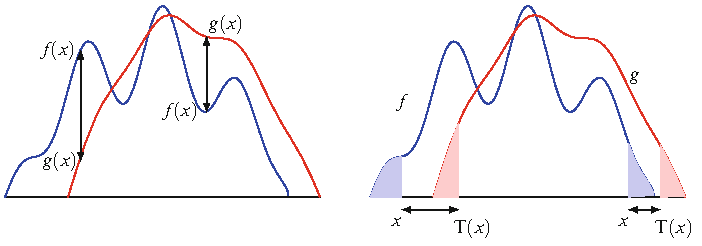
\includegraphics[width=\linewidth]{assets/ch05-fig-5-1.pdf}
\caption{“竖直”距离与“水平”距离（右图中的运输$\mathrm T$按一维情形计算，要求$f$与$g$图像下的蓝色、红色区域面积相等，也就是像\autoref{sec:2}那样使用CFD函数）.}\label{fig:5.1}
\end{figure}

在若干应用中，Wasserstein距离对于密度扰动的这种稳健性，使它们比其他距离更适合使用；而它们能度量测度的空间特征，恰好也是所需的. 此外，将在\autoref{sec:5.4}，以及后面的\autoref{sec:6.1}与\autoref{sec:7.3}看到，这些距离的测地线给出了质量分布之间有用的插值.

\subsection{定义与三角不等式}\label{sec:5.1}\index{W159@Wasserstein距离（Wasserstein distance）|hyperpage}

本节给出$\Omega\subset\mathbb R^d$中Wasserstein距离与空间的基本定义. 将看到如何把分析调整到更一般的度量空间情形. 如上所述，将分析限制于集合
\[
\mathscr P_p(\Omega):=\left\{\mu\in\mathscr P(\Omega):\int|x|^p\,d\mu<+\infty\right\}.
\]
注意，$p<q$蕴含$\mathscr P_p(\Omega)\subset\mathscr P_q(\Omega)$；而只要$\Omega$有界，就有$\mathscr P_p(\Omega)=\mathscr P(\Omega)$.

对$\mu,\nu\in\mathscr P_p(\Omega)$，定义
\[
W_p(\mu,\nu):=\min\left\{\int_{\Omega\times\Omega}|x-y|^p\,d\gamma:\gamma\in\Pi(\mu,\nu)\right\}^{1/p},
\]
即成本$c(x,y)=|x-y|^p$的最小运输成本$\mathscr T_c$的$p$次方根. 假设$\mu,\nu\in\mathscr P_p(\Omega)$保证该值有限，因为$|x-y|^p\le C(|x|^p+|y|^p)$，从而
$W_p^p(\mu,\nu)\le C(\int|x|^p\,d\mu+\int|x|^p\,d\nu)$.

注意，由Jensen不等式，由于所有$\gamma\in\Pi(\mu,\nu)$均为概率测度，对$p\le q$有
\[
\left(\int|x-y|^p\,d\gamma\right)^{1/p}
=\|x-y\|_{L^p(\gamma)}\le\|x-y\|_{L^q(\gamma)}
=\left(\int|x-y|^q\,d\gamma\right)^{1/q},
\]
这蕴含$W_p(\mu,\nu)\le W_q(\mu,\nu)$. 特别地，对每个$p\ge1$，都有$W_1(\mu,\nu)\le W_p(\mu,\nu)$. 这里不定义$W_\infty$；其作为$p\to\infty$的极限的定义见\autoref{sec:5.5.1}.

另一方面，当$\Omega$有界时，反向不等式也成立，因为
\[
\left(\int|x-y|^p\,d\gamma\right)^{1/p}
\le\operatorname{diam}(\Omega)^{(p-1)/p}\left(\int|x-y|\,d\gamma\right)^{1/p}.
\]
这蕴含
\begin{equation}\label{eq:5.1}
W_p(\mu,\nu)\le C W_1(\mu,\nu)^{1/p},
\end{equation}
其中$C=\operatorname{diam}(\Omega)^{(p-1)/p}$.

\begin{proposition}\label{obj:5.1}
上述量$W_p$是$\mathscr P_p(\Omega)$上的距离.
\end{proposition}
\begin{proof}
首先，$W_p\ge0$. 还注意到，$W_p(\mu,\nu)=0$蕴含存在$\gamma\in\Pi(\mu,\nu)$，使$\int|x-y|^p\,d\gamma=0$. 这样的$\gamma\in\Pi(\mu,\nu)$集中于$\{x=y\}$上. 这蕴含$\mu=\nu$，因为对任意测试函数$\phi$，有
\[
\int\phi\,d\mu=\int\phi(x)\,d\gamma=\int\phi(y)\,d\gamma=\int\phi\,d\nu.
\]
现在需要证明三角不等式. 对此给出两个不同的证明. 第一个（\autoref{obj:5.3}）较容易，使用运输映射和逼近；第二个（\autoref{obj:5.4}）更一般，但需要较复杂的工具，即测度分解.
\end{proof}

\begin{lemma}\label{obj:5.2}
给定$\mu,\nu\in\mathscr P_p(\mathbb R^d)$，以及任意$L^1$中的偶正则化核$\chi_\varepsilon$，满足$\int_{\mathbb R^d}\chi_\varepsilon(z)\,dz=1$与$\chi_\varepsilon(z)=\varepsilon^{-d}\chi_1(z/\varepsilon)$，则有：
\begin{enumerate}
\item 不等式$W_p(\mu*\chi_\varepsilon,\nu*\chi_\varepsilon)\le W_p(\mu,\nu)$；
\item 极限$\lim_{\varepsilon\to0}W_p(\mu*\chi_\varepsilon,\nu*\chi_\varepsilon)=W_p(\mu,\nu)$.
\end{enumerate}
\end{lemma}
\begin{proof}
取最优运输方案$\gamma\in\Pi(\mu,\nu)$，通过
\[
\int_{\mathbb R^d\times\mathbb R^d}\phi(x,y)\,d\gamma_\varepsilon
:=\int_{\mathbb R^d\times\mathbb R^d}\int_{\mathbb R^d}\phi(x+z,y+z)\chi_\varepsilon(z)\,dz\,d\gamma(x,y)
\]
定义运输方案$\gamma_\varepsilon\in\Pi(\mu*\chi_\varepsilon,\nu*\chi_\varepsilon)$.
需验证它的边缘测度确实为$\mu*\chi_\varepsilon$与$\nu*\chi_\varepsilon$. 只需考虑
\[
\begin{aligned}
\int_{\mathbb R^d\times\mathbb R^d}\phi(x)\,d\gamma_\varepsilon
&=\int_{\mathbb R^d\times\mathbb R^d}\int_{\mathbb R^d}\phi(x+z)\chi_\varepsilon(z)\,dz\,d\gamma(x,y)\\
&=\int_{\mathbb R^d\times\mathbb R^d}(\phi*\chi_\varepsilon)(x)\,d\gamma(x,y)\\
&=\int_{\mathbb R^d}(\phi*\chi_\varepsilon)(x)\,d\mu(x)
=\int_{\mathbb R^d}\phi(x)\,d(\mu*\chi_\varepsilon)(x)
\end{aligned}
\]
（利用$\chi_\varepsilon$为偶函数，将卷积从$\phi$转移到$\mu$）. 第二个边缘测度的计算相同. 然后容易说明$\int|x-y|^p\,d\gamma_\varepsilon=\int|x-y|^p\,d\gamma$，因为
\[
\begin{aligned}
\int|x-y|^p\,d\gamma_\varepsilon
&=\int_{\mathbb R^d\times\mathbb R^d}\int_{\mathbb R^d}|(x+z)-(y+z)|^p\chi_\varepsilon(z)\,dz\,d\gamma(x,y)\\
&=\int|x-y|^p\,d\gamma.
\end{aligned}
\]
这说明第一部分，也说明
\[
\limsup_{\varepsilon\to0}W_p(\mu*\chi_\varepsilon,\nu*\chi_\varepsilon)^p
\le\limsup_{\varepsilon\to0}\int|x-y|^p\,d\gamma_\varepsilon=\int|x-y|^p\,d\gamma.
\]
反向不等式可用标准半连续性论证得到. 考虑$\mu_\varepsilon:=\mu*\chi_\varepsilon$、$\nu_\varepsilon:=\nu*\chi_\varepsilon$，只利用弱收敛$\mu_\varepsilon\rightharpoonup\mu$与$\nu_\varepsilon\rightharpoonup\nu$. 将$\Pi(\mu_\varepsilon,\nu_\varepsilon)$中的最优方案记为$\overline\gamma_\varepsilon$. 由于边缘测度紧，这列方案也紧（见\autoref{obj:1.7}的证明）. 先固定一列$\varepsilon_k\to0$，使$\lim_kW_p(\mu_{\varepsilon_k},\nu_{\varepsilon_k})=\liminf_{\varepsilon\to0}W_p(\mu_\varepsilon,\nu_\varepsilon)$. 再取子列$\varepsilon_{k_j}$，保证最优方案$\overline\gamma_{\varepsilon_{k_j}}$有弱极限$\overline\gamma_0$. 这一弱极限必属于$\Pi(\mu,\nu)$（其边缘测度为$\mu$与$\nu$，来自弱收敛与连续函数复合的性质）. 于是
\[
\begin{aligned}
W_p^p(\mu,\nu)&\le\int|x-y|^p\,d\overline\gamma_0
\le\liminf_j\int|x-y|^p\,d\overline\gamma_{\varepsilon_{k_j}}\\
&=\liminf_{\varepsilon\to0}W_p(\mu_\varepsilon,\nu_\varepsilon),
\end{aligned}
\]
其中第一个不等式来自$\overline\gamma_0$虽不一定最优却可容许，第二个则来自半连续性（\autoref{obj:1.6}）.
\end{proof}

现在可基于最优运输映射，证明三角不等式.

\begin{lemma}\label{obj:5.3}\index{W159@Wasserstein距离（Wasserstein distance）!160@三角不等式（triangle inequality）|hyperpage}
量$W_p$满足三角不等式（利用运输映射与逼近的证明）.
\end{lemma}
\begin{proof}
先考虑$\mu$与$\varrho$绝对连续、$\nu$任意的情形. 设$\mathrm T$为从$\mu$到$\varrho$的最优运输，$S$为从$\varrho$到$\nu$的最优运输. 则$S\circ\mathrm T$是从$\mu$到$\nu$的可容许运输，因为$(S\circ\mathrm T)_\#\mu=S_\#(\mathrm T_\#\mu)=S_\#\varrho=\nu$. 有
\[
\begin{aligned}
W_p(\mu,\nu)&\le\left(\int|S(\mathrm T(x))-x|^p\,d\mu(x)\right)^{1/p}
=\|S\circ\mathrm T-\mathrm{id}\|_{L^p(\mu)}\\
&\le\|S\circ\mathrm T-\mathrm T\|_{L^p(\mu)}+\|\mathrm T-\mathrm{id}\|_{L^p(\mu)}.
\end{aligned}
\]
此外，
\[
\begin{aligned}
\|S\circ\mathrm T-\mathrm T\|_{L^p(\mu)}
&=\left(\int|S(\mathrm T(x))-\mathrm T(x)|^p\,d\mu(x)\right)^{1/p}\\
&=\left(\int|S(y)-y|^p\,d\varrho(y)\right)^{1/p},
\end{aligned}
\]
最后这一量等于$W_p(\varrho,\nu)$. 又有$\|\mathrm T-\mathrm{id}\|_{L^p(\mu)}=W_p(\mu,\varrho)$，因而
\[
W_p(\mu,\nu)\le W_p(\mu,\varrho)+W_p(\varrho,\nu).
\]
这就证明了$\mu,\varrho\ll\mathscr L^d$的情形. 对一般情形，先对$\mu*\chi_\varepsilon$、$\varrho*\chi_\varepsilon$与$\nu*\chi_\varepsilon$写出三角不等式，再利用\autoref{obj:5.2}令$\varepsilon\to0$即可.
\end{proof}

上述证明大量使用了\autoref{sec:1}关于运输映射的结果，在某种意义上是$\mathbb R^d$所特有的（在一般度量空间中，困难在于用这样一些测度逼近任意测度：它们之间的Wasserstein距离可用映射而非方案计算\footnote{严格说不必使用绝对连续测度：实际只需无原子测度，然后可应用\autoref{obj:1.33}.}）. 为给出更一般的结果，再提供另一种证明；对不熟悉测度分解的读者（见\autoref{sec:2}），它可能更难一些.

\begin{lemma}\label{obj:5.4}\index{D041@测度的分解（disintegration of measures）|hyperpage}\index{W159@Wasserstein距离（Wasserstein distance）!160@三角不等式（triangle inequality）|hyperpage}
量$W_p$满足三角不等式（利用测度分解的证明）.
\end{lemma}
\begin{proof}
取$\mu,\varrho,\nu\in\mathscr P_p(\Omega)$，$\gamma^+\in\Pi(\mu,\varrho)$与$\gamma^-\in\Pi(\varrho,\nu)$. 还可以选择$\gamma^\pm$最优. 由\autoref{obj:5.5}，存在测度$\sigma\in\mathscr P(\Omega\times\Omega\times\Omega)$使$(\pi_{x,y})_\#\sigma=\gamma^+$与$(\pi_{y,z})_\#\sigma=\gamma^-$，其中$\pi_{x,y}$、$\pi_{y,z}$分别表示到前两个与后两个变量的投影. 取$\gamma:=(\pi_{x,z})_\#\sigma$. 通过投影复合，容易看出$(\pi_x)_\#\gamma=(\pi_x)_\#\sigma=(\pi_x)_\#\gamma^+=\mu$，同样有$(\pi_z)_\#\gamma=\nu$. 这意味着$\gamma\in\Pi(\mu,\nu)$，且
\[
\begin{aligned}
W_p(\mu,\nu)&\le\left(\int|x-z|^p\,d\gamma\right)^{1/p}
=\left(\int|x-z|^p\,d\sigma\right)^{1/p}=\|x-z\|_{L^p(\sigma)}\\
&\le\|x-y\|_{L^p(\sigma)}+\|y-z\|_{L^p(\sigma)}\\
&=\left(\int|x-y|^p\,d\sigma\right)^{1/p}+\left(\int|y-z|^p\,d\sigma\right)^{1/p}\\
&=\left(\int|x-y|^p\,d\gamma^+\right)^{1/p}+\left(\int|y-z|^p\,d\gamma^-\right)^{1/p}\\
&=W_p(\mu,\varrho)+W_p(\varrho,\nu).
\end{aligned}
\]
证明完成.
\end{proof}

下面的引理通常称为“黏合引理”（gluing lemma），它使两个运输方案可以像映射一样作某种“复合”.

\begin{lemma}\label{obj:5.5}\index{G070@粘合引理（gluing lemma）|hyperpage}
给定两个测度$\gamma^+\in\Pi(\mu,\varrho)$与$\gamma^-\in\Pi(\varrho,\nu)$，至少存在一个测度$\sigma\in\mathscr P(\Omega\times\Omega\times\Omega)$，使$(\pi_{x,y})_\#\sigma=\gamma^+$与$(\pi_{y,z})_\#\sigma=\gamma^-$，其中$\pi_{x,y}$、$\pi_{y,z}$分别表示到前两个与后两个变量的投影.
\end{lemma}
\begin{proof}
先取$\gamma^+$，关于投影$\pi_y$进行分解（见\autoref{sec:2.3}的\autoref{box:2.2}）. 得到一族测度$\gamma_y^+\in\mathscr P(\Omega)$（如该框所指出，可将它们视为$\Omega$上的测度，而不视为$\Omega\times\{y\}\subset\Omega\times\Omega$上的测度）. 对每个二元可测函数$\phi$，它们满足（实际上由下式定义）
\[
\int_{\Omega\times\Omega}\phi(x,y)\,d\gamma^+(x,y)
=\int_\Omega d\varrho(y)\int_\Omega\phi(x,y)\,d\gamma_y^+(x).
\]
同样，有一族测度$\gamma_y^-\in\mathscr P(\Omega)$，对每个$\phi$满足
\[
\int_{\Omega\times\Omega}\phi(y,z)\,d\gamma^-(y,z)
=\int_\Omega d\varrho(y)\int_\Omega\phi(y,z)\,d\gamma_y^-(z).
\]
对每个$y$，取$\Omega\times\Omega$上的测度$\gamma_y^+\otimes\gamma_y^-$. 通过
\[
\int_{\Omega\times\Omega\times\Omega}\phi(x,y,z)\,d\sigma(x,y,z)
:=\int_\Omega d\varrho(y)\int_{\Omega\times\Omega}\phi(x,y,z)\,d(\gamma_y^+\otimes\gamma_y^-)(x,z)
\]
定义$\sigma$. 容易验证，若$\phi$只依赖于$x$与$y$，则
\[
\begin{aligned}
\int_{\Omega^3}\phi(x,y)\,d\sigma
&=\int_\Omega d\varrho(y)\int_{\Omega\times\Omega}\phi(x,y)\,d(\gamma_y^+\otimes\gamma_y^-)(x,z)\\
&=\int_\Omega d\varrho(y)\int_\Omega\phi(x,y)\,d\gamma_y^+(x)=\int\phi\,d\gamma^+.
\end{aligned}
\]
这证明了$(\pi_{x,y})_\#\sigma=\gamma^+$；$(\pi_{y,z})_\#\sigma=\gamma^-$的证明类似.
\end{proof}

\begin{remark}\label{obj:5.6}\index{P114@Polish空间（Polish spaces）|hyperpage}
本节的全部分析都可以在一般Polish空间$X$上进行，而不限于子集$\Omega\subset\mathbb R^d$. 唯一区别是$\mathscr P_p(X)$的定义（需要使用$\mathscr P_p(X):=\{\mu\in\mathscr P(X):\int d(x,x_0)^p\,d\mu(x)<+\infty\}$），以及三角不等式的第一个证明是$\mathbb R^d$所特有的（但第二个一般适用）.
\end{remark}

\begin{definition}\label{obj:5.7}\index{W159@Wasserstein距离（Wasserstein distance）!161@Wasserstein空间（Wasserstein spaces）|hyperpage}
给定Polish空间$X$，对每个$p\in[1,+\infty[$，将其\emph{$p$阶Wasserstein空间}$\mathbb W_p(X)$定义为赋予距离$W_p$的空间$\mathscr P_p(X)$.
\end{definition}
